\subsection{HWP non uniform optical properties}

\paragraph{Description:}
Non-uniformities (e.g.: small patches of the HWP surface with lower or higher transmission/reflection/absorption with respect to the overall surface) in the optical properties produce discontinuities in the output signal.

This is expected to be relatively small, but we should model it to check, especially if the
HWP is in an optical position where detectors don’t see the same HWP.

\paragraph{Plan to model and/or measure:}
Different approaches can be used to study this systematics:
EM calculation with gap (or dust) between layers or thickness error,
3D shape measurement/FTS measurements for various points on HWP and, finally, investigation of the
HWP synchronous signal.

\paragraph{Uncertainty/Range:}
Uncertainty could come from many aspects:
optical index, geometry, distribution and beam convolution.

\paragraph{Parameterization:}
The simplest way is to introduce a discontinuous variation in one HWP optical property;
in a test model we have introduced a 10$\%$ increase of the extraordinary index when the HWP
is rotating at 36deg (Fig.\,\ref{}).


%SRF: 3*,

%\begin{figure}
%\centering
%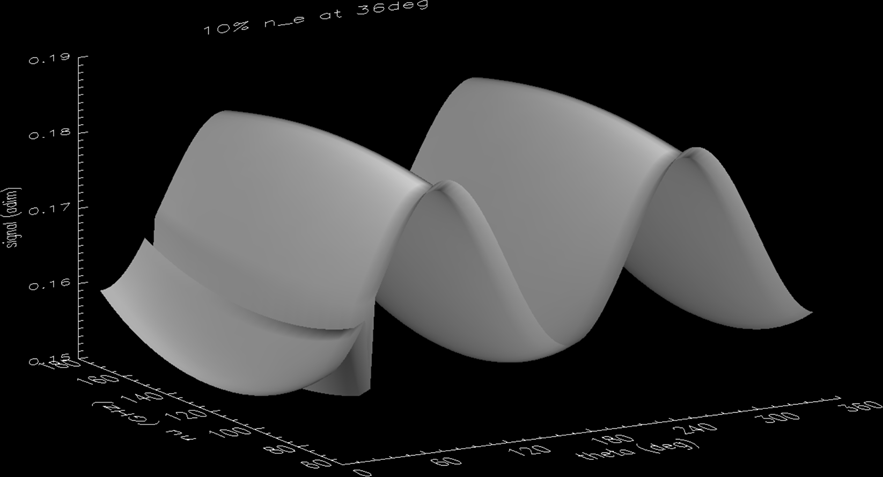
\includegraphics[width=2.5in]{figures/hwp_nonuniform.png}
%\caption{2$f$ signal from a (1,0,0,0) Stokes vector incident on a HWP with a localized non-uniformity: a discontinuous increase of
%10$\%$ of the extraordinary index at theta=36${\circ}$}.}\label{hwpnonuniform}
%\end{figure}
